\documentclass{article}
\usepackage[section]{placeins}
\usepackage{graphicx, wrapfig, amsmath, amssymb, physics, hyperref}
\hypersetup{
    colorlinks=true,
    linkcolor=blue,
    filecolor=magenta,      
    urlcolor=cyan,
    }

\author{Yaghoub Shahmari}
\title{Report - Problem Set No 10}
\date{\today}
\graphicspath{ {../Figs/} }

\begin{document}
    \maketitle
    \section*{Basic description}

    In this problem, we want to simulate a system containing molecules and periodic boundaries. For the interaction between molecules, we consider Leonard-jones potential:

    $$u\left(r_{i j}\right)= \begin{cases}4 \epsilon\left[\left(\frac{\sigma}{r_{i j}}\right)^{12}-\left(\frac{\sigma}{r_{i j}}\right)^{6}\right] & r_{i j}<r_{c} \\ 0 & r_{i j} \geq r_{c}\end{cases}$$

    Where $\textbf{r}_{ij} = \textbf{r}_i - \textbf{r}_j\ and\ r_{ij} = |\textbf{r}_{ij}|$. Thanks to the above relation, we can find the potential energy. To find force, kinetic energy, pressure, and temperature we can use the following relation:

    $$
    \begin{gathered}
    f_{i j}=\left(\frac{48 \epsilon}{\sigma^{2}}\right)\left[\left(\frac{\sigma}{r_{i j}}\right)^{14}-\frac{1}{2}\left(\frac{\sigma}{r_{i j}}\right)^{8}\right] \boldsymbol{r}_{i j} \\
    E_{K}=\frac{1}{2} \sum_{i=1}^{N_{m}} \boldsymbol{v}_{i}^{2} \\
    E_{U}=4 \sum_{1 \leq i<j \leq N_{m}}\left(r_{i j}^{-12}-r_{i j}^{-6}\right) \\
    T=\frac{1}{d N_{m}} \sum_{i} \boldsymbol{v}_{i}^{2} \\
    P V=\frac{1}{d}\left\langle\sum_{i} \boldsymbol{v}_{i}^{2}+48 \sum_{i<j}\left(r_{i j}^{-12}-\frac{1}{2} r_{i j}^{-6}\right)\right\rangle
    \end{gathered}
    $$

    To reduce the computations, we consider all of the reduced units as one. Also, RC is equal to half the length of the system side.
    
    \pagebreak

    \section*{Trajectory}

    In the animation folder, there are two animations of simulations.
    One is for simulation of Argon gas, and the other is for temperature drop, which contains phase transmission trajectory.
    Related charts are provided later.

    \section*{Equilibrium}

    To find the properties of a system in equilibrium, I simulated a single system of molecules with a given initial condition and continued the simulation for a while after equilibrium.
    The initial positions of molecules follow the crystal structure.

    \subsection*{The results:}

    \begin{figure}[!htb]
        \centering
        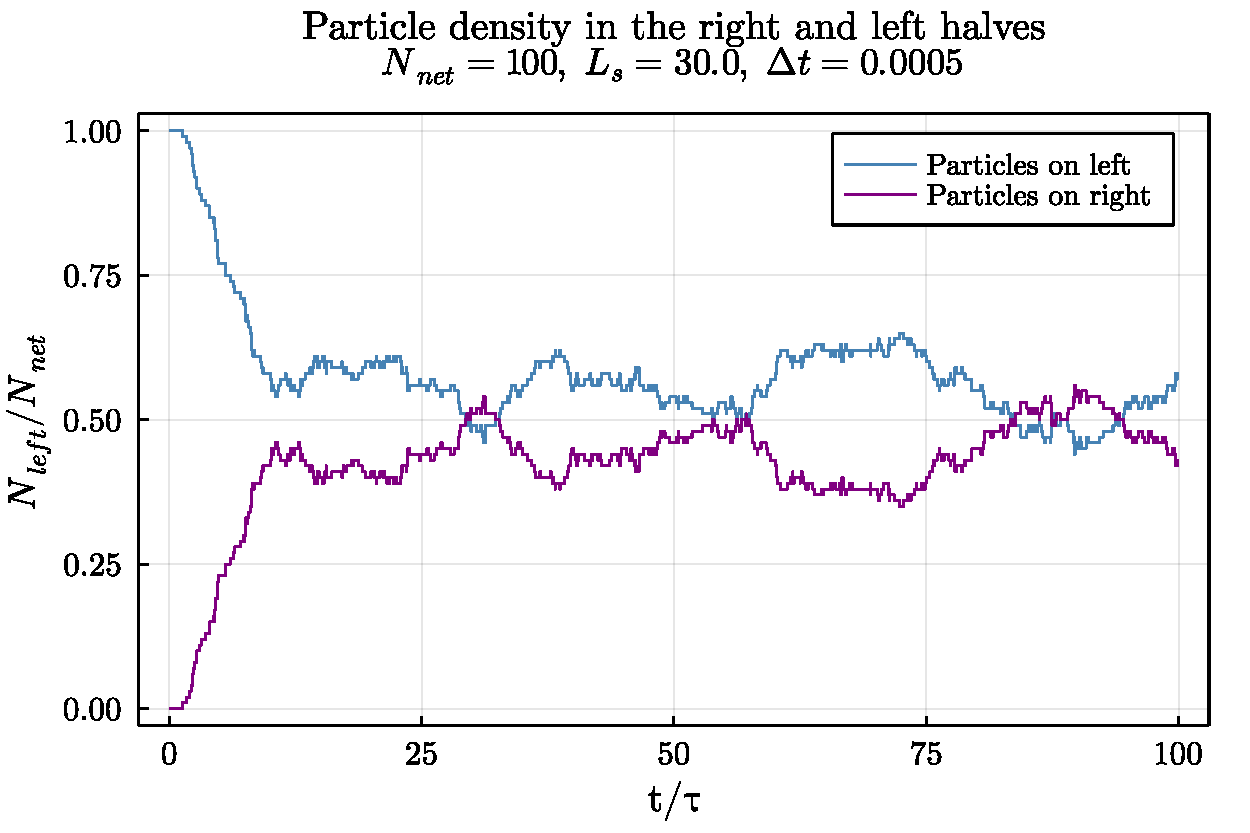
\includegraphics[scale = 0.3]{/Fig1}
        \label{fig.1}
        \caption{Diagram of proportion of particles on each side of the system can be a criterion of homogeneity of the system and can show us equilibrium.}
    \end{figure}

    \begin{figure}[!htb]
        \centering
        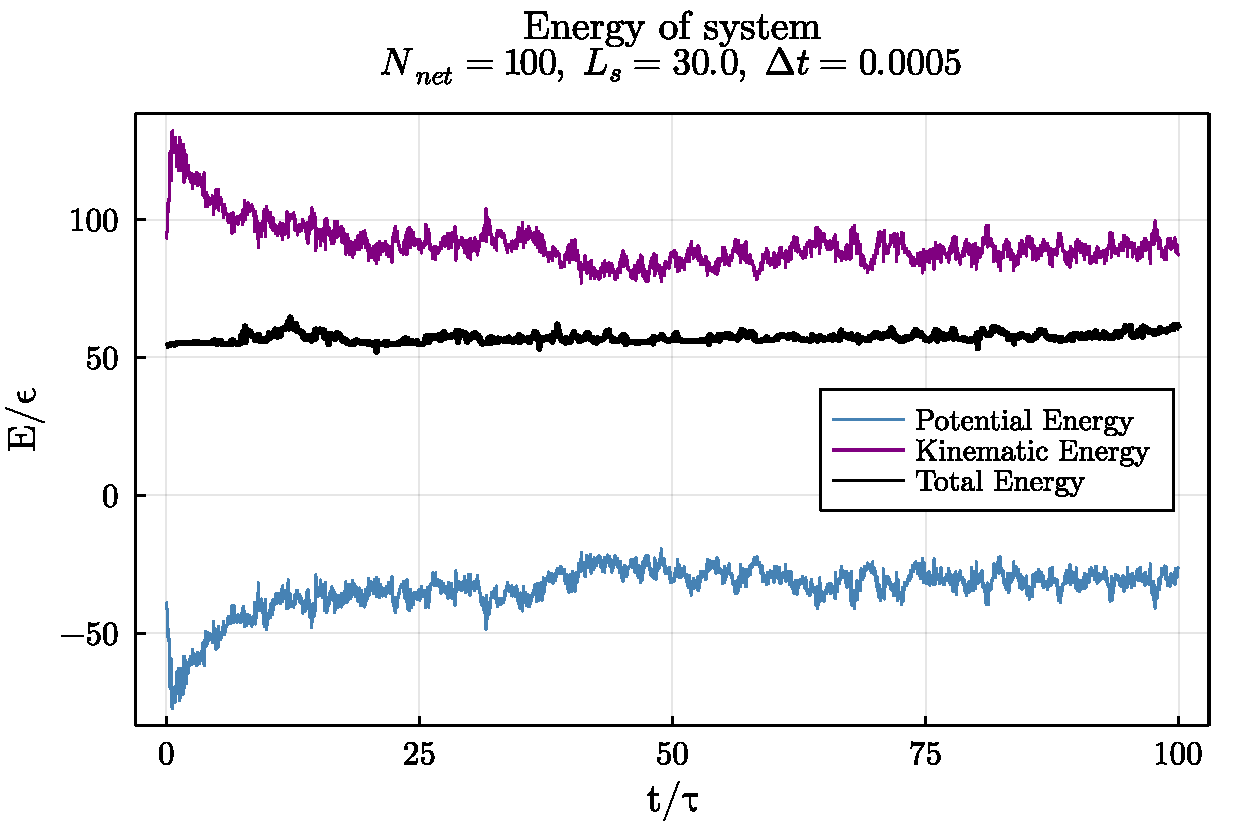
\includegraphics[scale = 0.3]{/Fig2}
        \label{fig.2}
        \caption{Diagram of kinetic energy, potential energy, and total energy of the system. As was expected, the total energy is almost constant.}
    \end{figure}

    \begin{figure}[!htb]
        \centering
        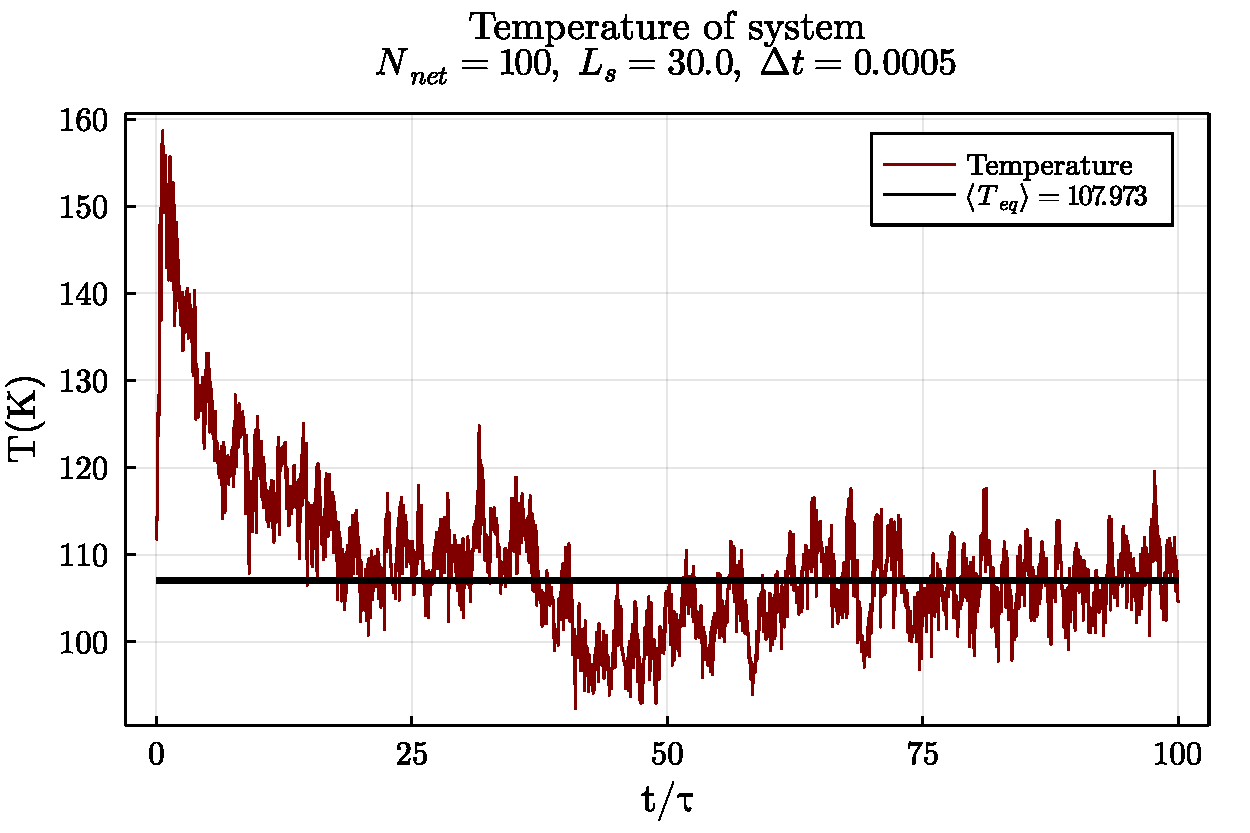
\includegraphics[scale = 0.25]{/Fig3}
        \label{fig.3}
        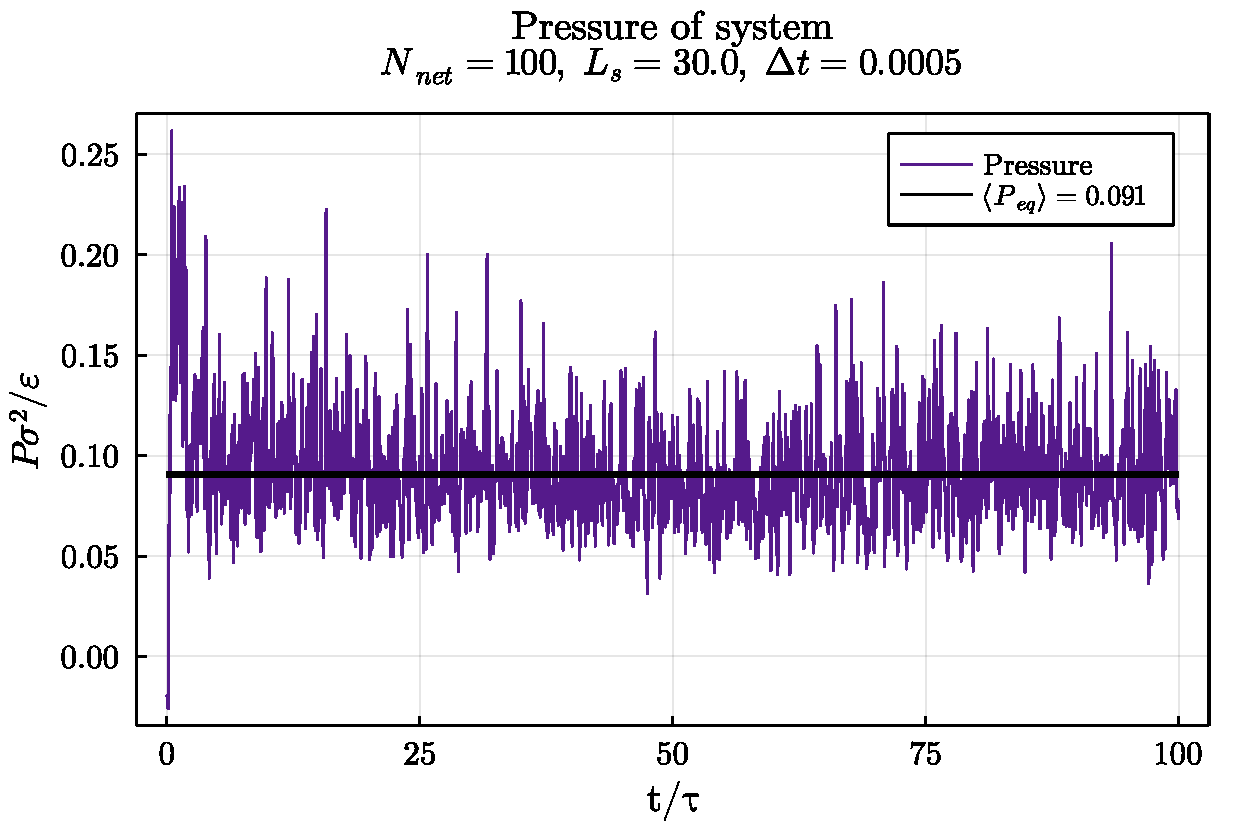
\includegraphics[scale = 0.25]{/Fig4}
        \label{fig.4}
        \caption{Diagram of temperature and pressure of the system.}
    \end{figure}

    \section*{Autocorrelation of velocity}
    
    Autocorrelation function for velocity shows us when the particles will be independent of their initial speed. Given the following relation, we can find the relaxation time if we fit the results on the below term:

    $$
    C_v(t) \approx e^{-t/\xi}\quad (\text{Where $\xi$ is the relaxation time})
    $$

    \begin{figure}[!htb]
        \centering
        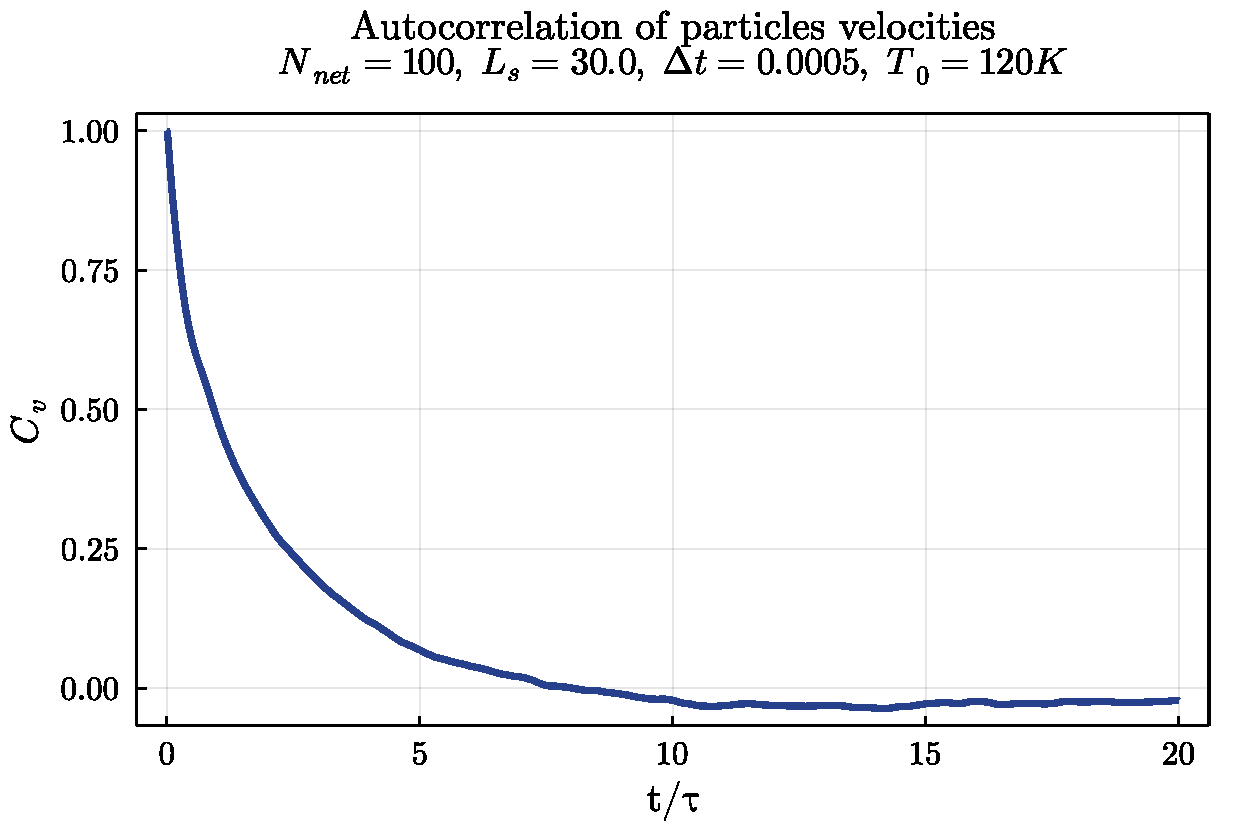
\includegraphics[scale = 0.5]{/Fig5}
        \label{fig.5}
        \caption{Diagram of autocorrelation of velocity for different times. As the result, $\xi = 1.604 \pm 0.0006$}
    \end{figure}

    \section*{Average on Properties of Systems}

    Yet we simulated a system of molecules in a single run.
    The results showed us the properties of the system in equilibrium.
    Due to the high number of steps, the value of properties in equilibrium was accurate.
    But due to the stochasticity of the system, there are noises that won't let us see the behavior of the system before that.
    So I also did repeat all the previous works and gathered data of many runs.
    Then I averaged on them to remove the noises so we can see the behavior of the system in the times before equilibrium.

    \subsection*{The results:}

    \begin{figure}[!htb]
        \centering
        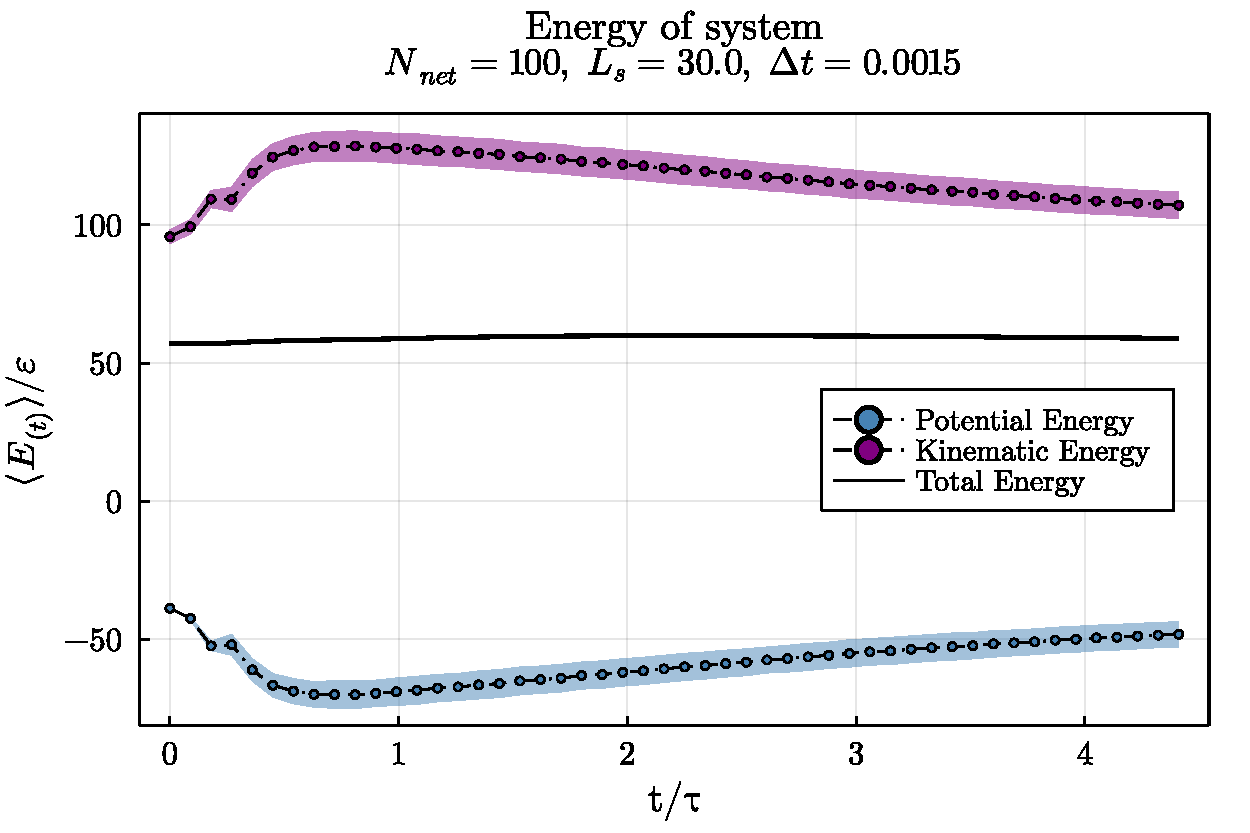
\includegraphics[scale = 0.5]{/Fig6}
        \label{fig.6}
        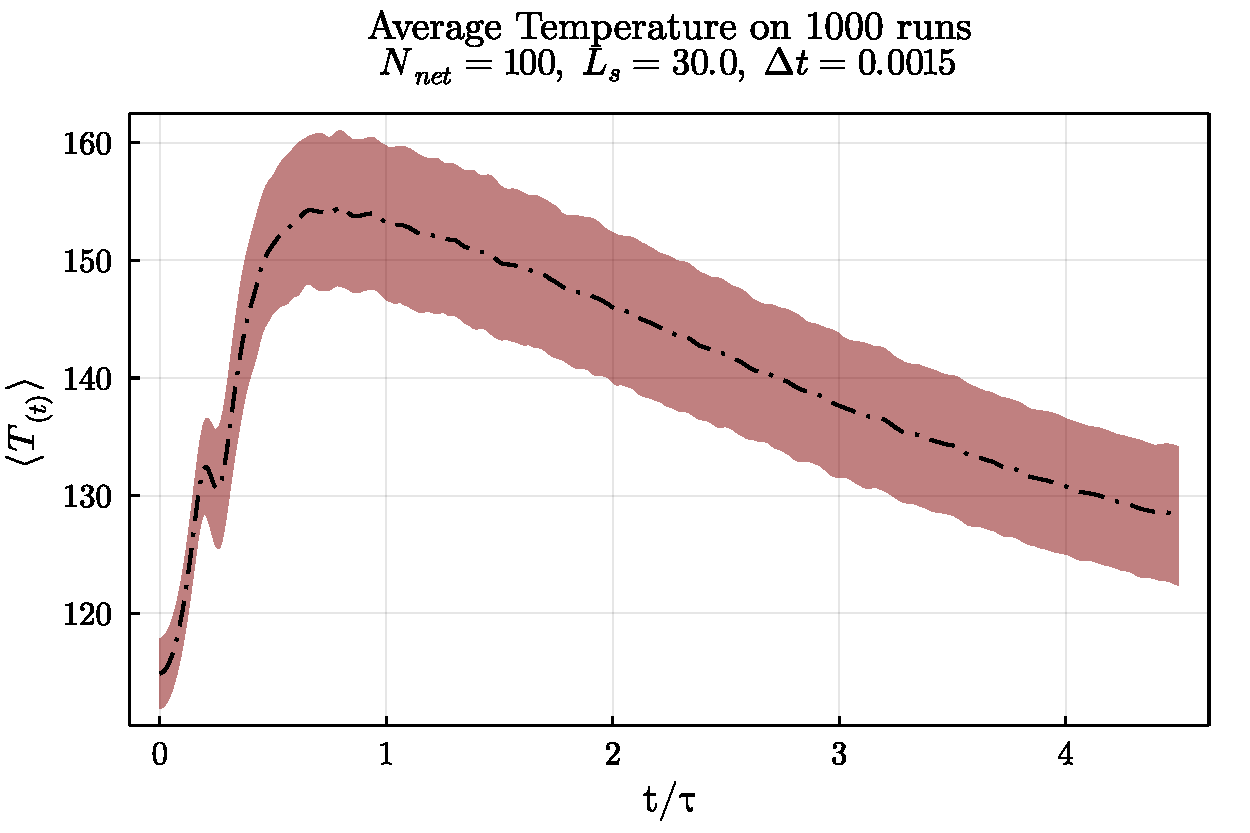
\includegraphics[scale = 0.25]{/Fig7}
        \label{fig.7}
        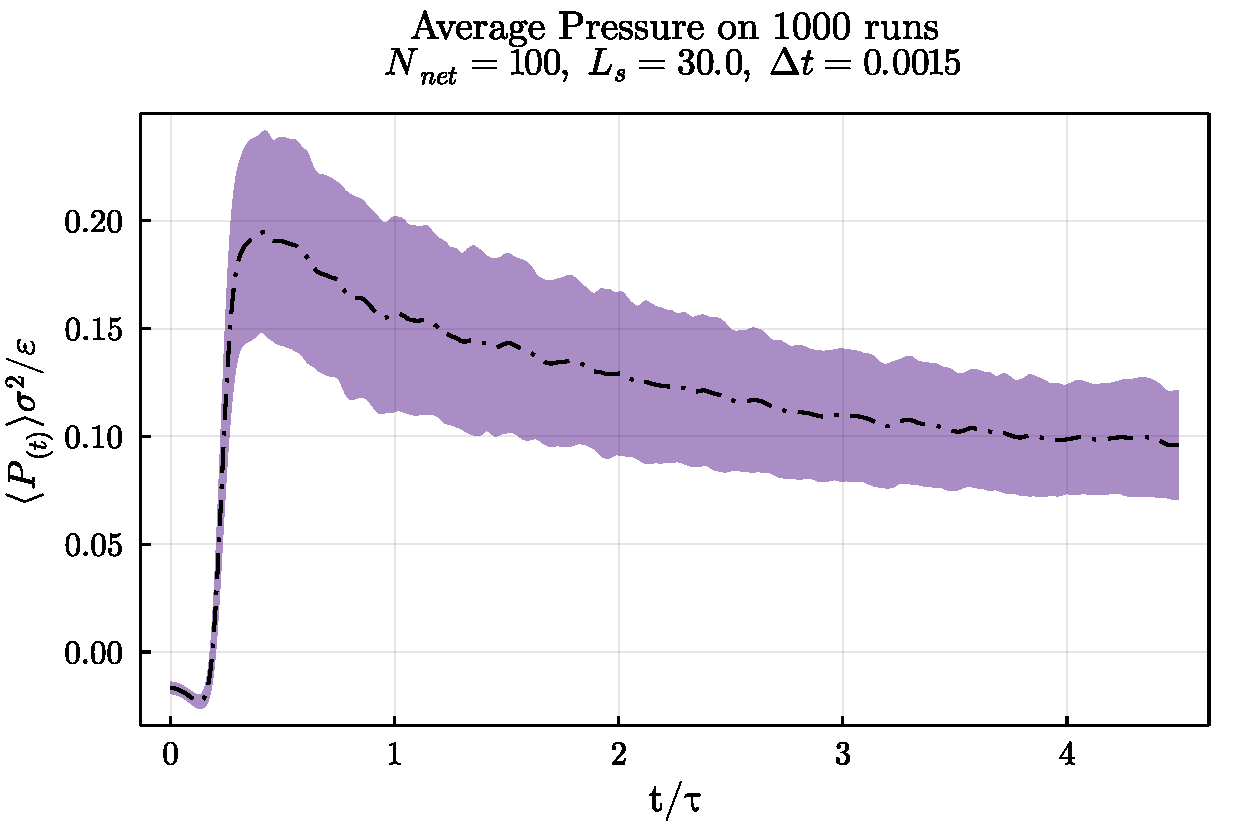
\includegraphics[scale = 0.25]{/Fig8}
        \label{fig.8}
        \caption{The average properties of the system.}
    \end{figure}

    \section*{Phase transmission}

    To see the phase transmission due to reducing temperature,
    I dropped the temperature of the system in a few stages by scaling the velocity of particles.
    The animation of the system is provided in the animation directory (I talked about it before),
    which shows the changing the phase of gas to liquid and solid.

    The diagrams that show more detail of the system during transmission are as follows:

    \begin{figure}[!htb]
        \centering
        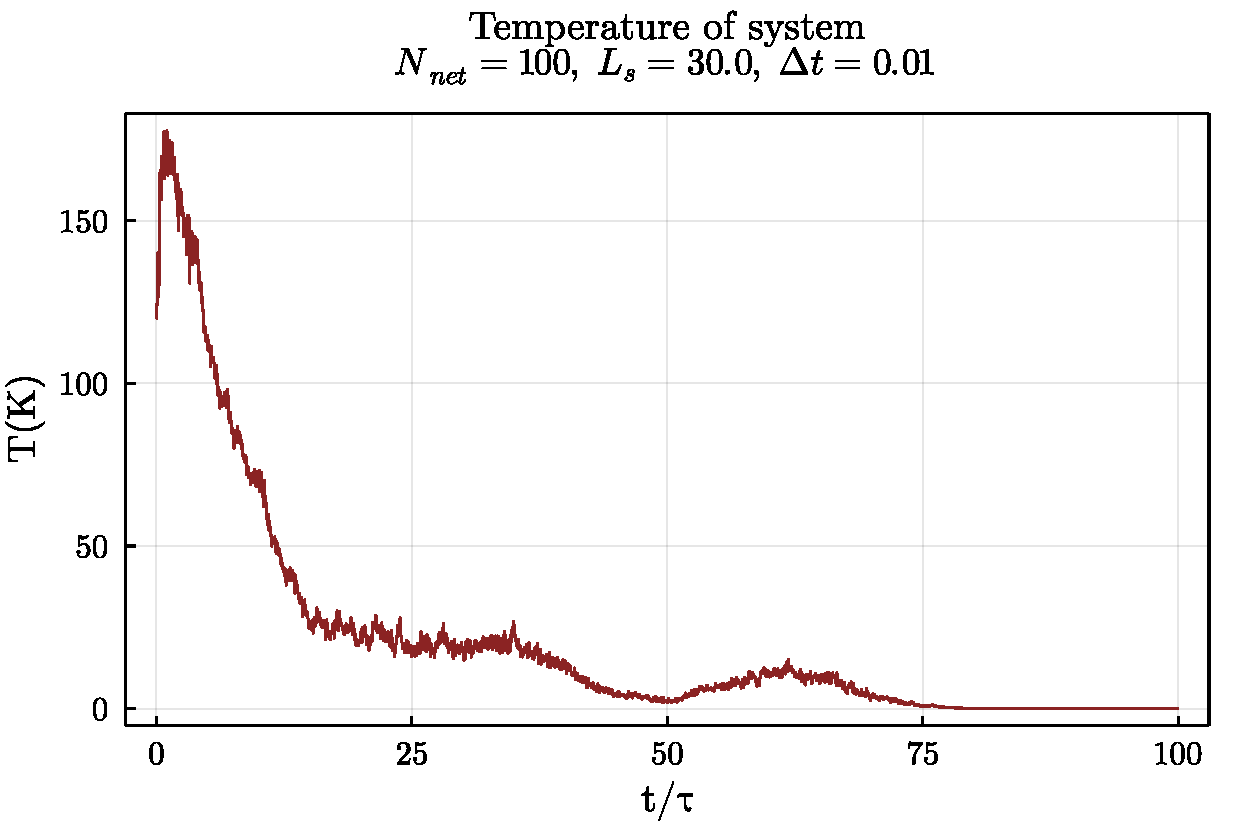
\includegraphics[scale = 0.25]{/Fig9}
        \label{fig.9}
        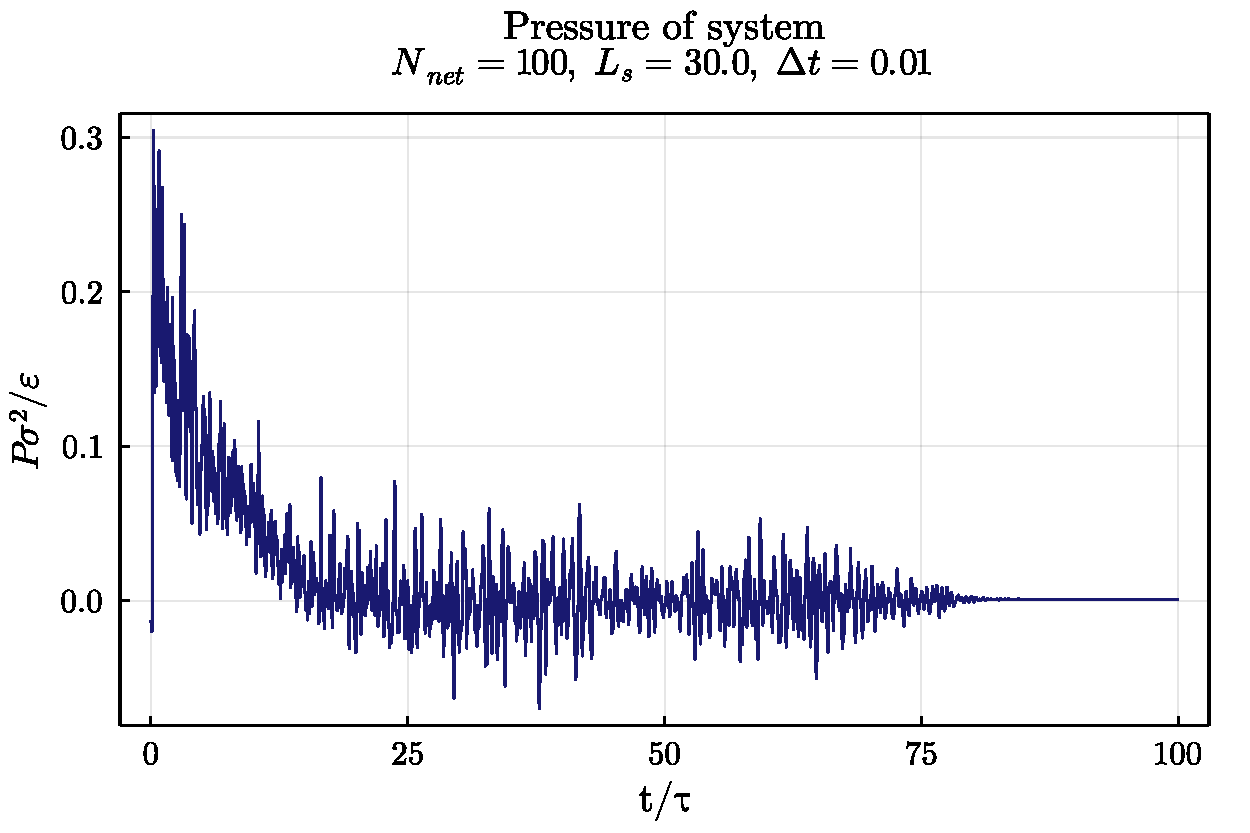
\includegraphics[scale = 0.25]{/Fig10}
        \label{fig.10}
        \caption{Diagram of temperature and pressure of the system.}
    \end{figure}

    \section*{Van der Waals Equation}

    The Van der Waals Equation is as follows:

    $$
    \left(P+a \frac{n^{2}}{V^{2}}\right)(V-n b)=n R T
    $$

    In our reduced units, it will show as following terms:

    $$
    P = A . T + B
    $$

    Where $A = \frac{1}{V/N - b^*}$ and $B = \frac{N^2}{V^2} a^*$.

    To export the data we need to find the coefficients,
    I took similar steps in the "Average on Properties of Systems" section but only averaged on the value of properties all of the times after equilibrium.
    The simple linear regression givies following results:

    $P = (0.13178 \pm 0.002025).T + (-0.02666 \pm 0.005643)$

    $$
    \Rightarrow \begin{cases}
        a^* \approx 2.16\\
        b^* \approx 1.41
    \end{cases}
    $$

    \begin{figure}[!htb]
        \centering
        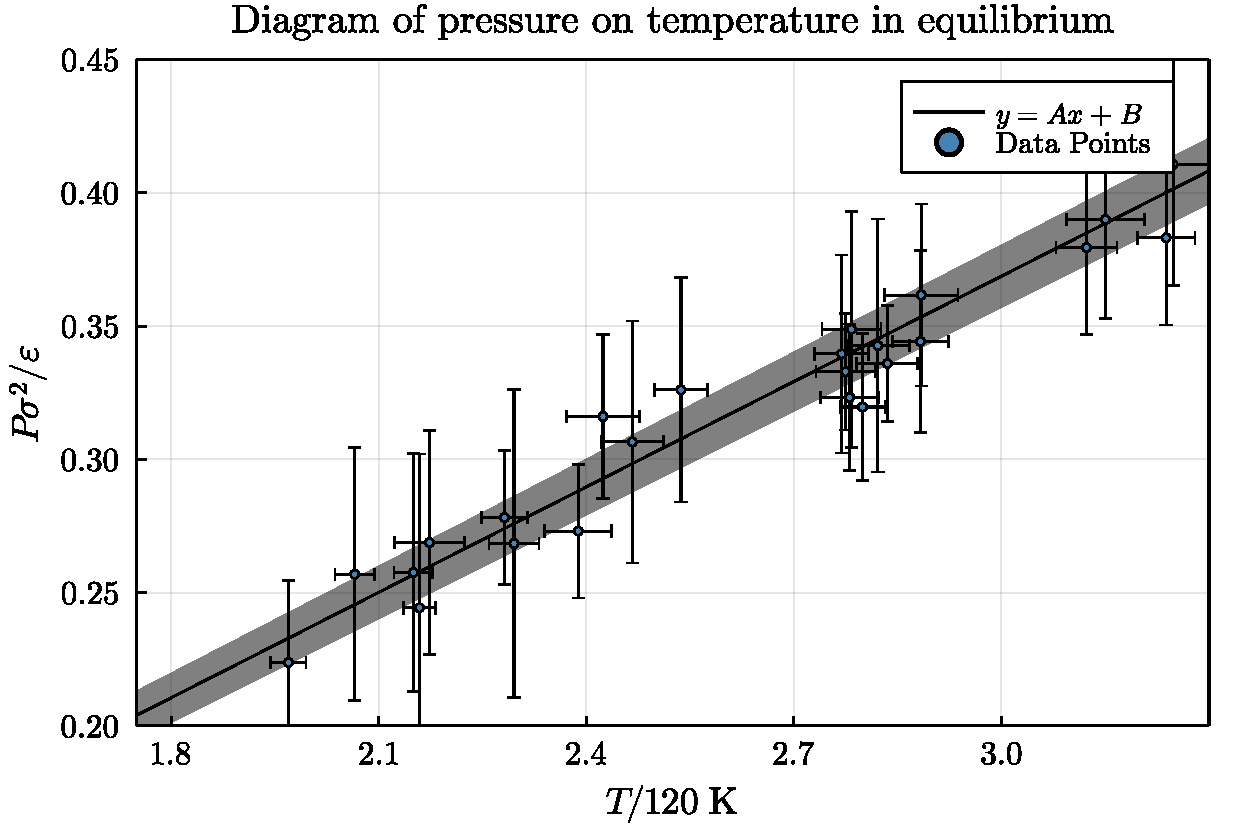
\includegraphics[scale = 0.5]{/Fig11}
        \label{fig.11}
        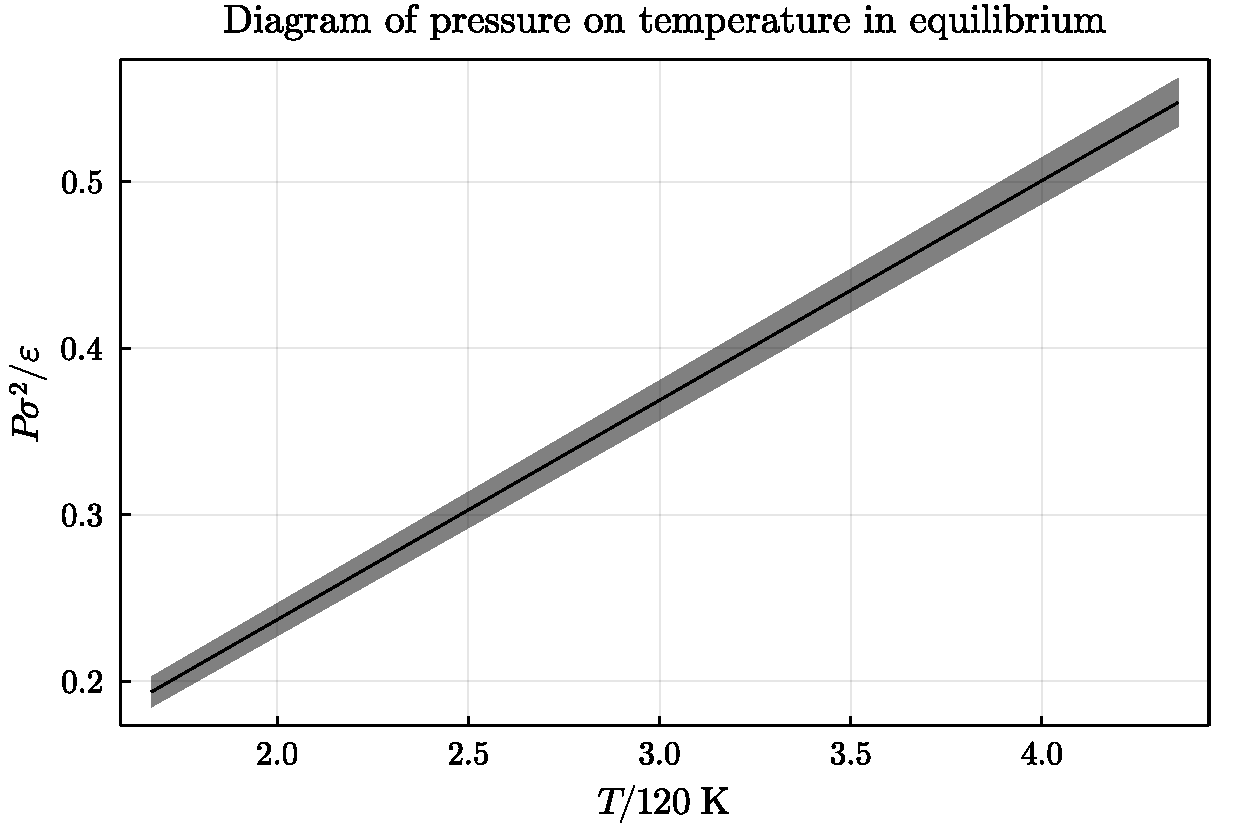
\includegraphics[scale = 0.25]{/Fig12}
        \label{fig.12}
        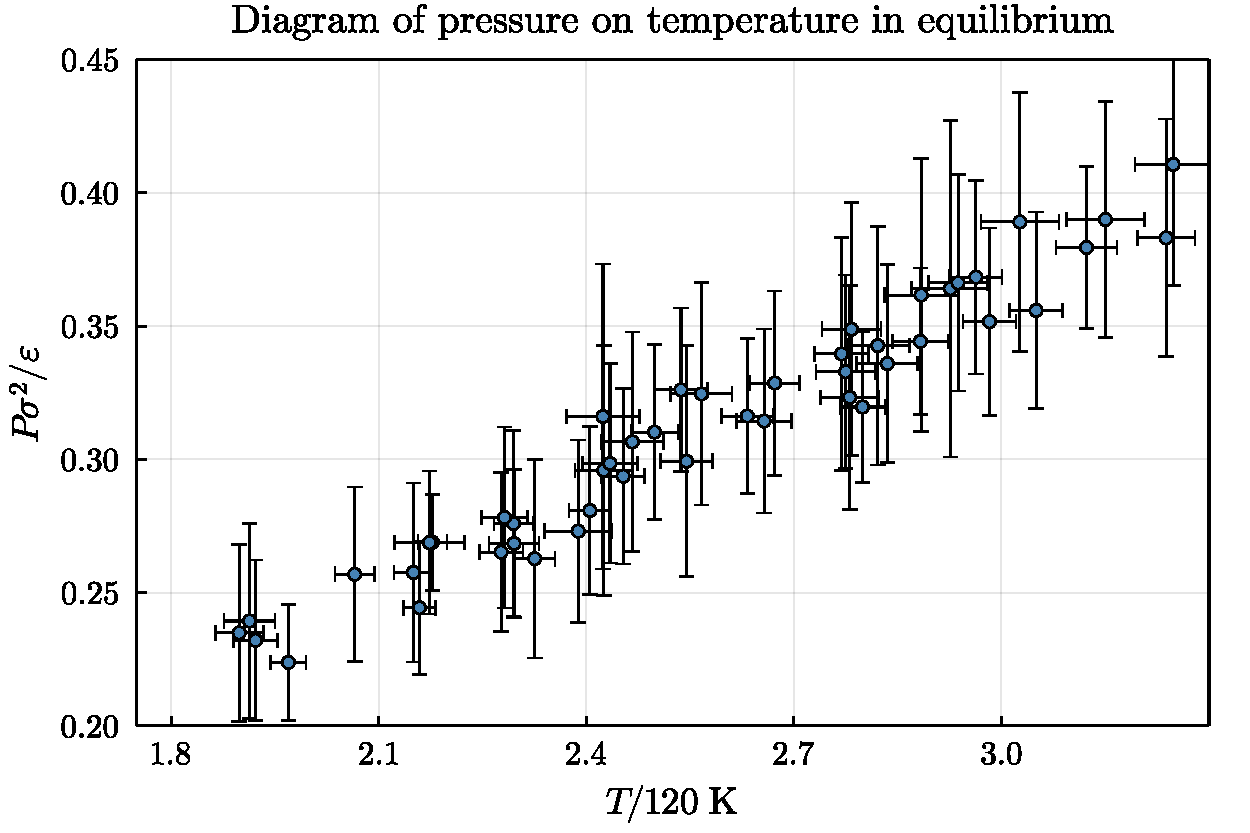
\includegraphics[scale = 0.25]{/Fig13}
        \label{fig.13}
        \caption{Diagram of mean pressures and temperatures at equilibrium. This points have equal energy. The line is result of simple linear regression of data.}
    \end{figure}

    \pagebreak

    \centering
    \textbf{The whole data I gathered is in \href{https://github.com/shahmari/ComputationalPhysics-Fall2021/tree/main/ProblemSet10/Data}{this link}}

    Thanks for watching :)
\end{document}